\section{Simulation Results}
The calculated properties from Molecular Dynamics simulations are presented 
in the following forms
\begin{figure}[h!]
    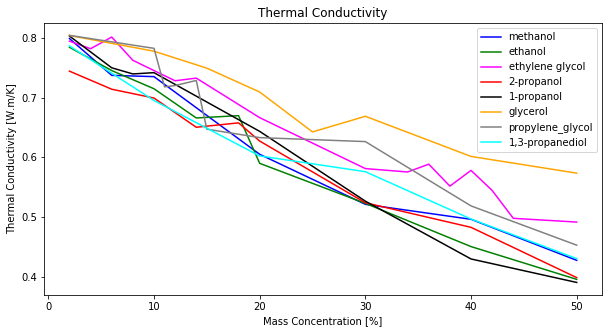
\includegraphics[width=1\textwidth]{tc.png}
    \centering
    \captionsetup{justification=centering}
    \caption{Thermal Conductivity Values of 8 Sample Alcohol Types Across Mass Concentration}
\end{figure}

As expected in the thermal conductivity graph, all the thermal conductivity 
lines decreased due to the fact that all types of alcohol are less efficient 
than water in terms of heat transfer. Even though having a decreasing trend, 
the gradient of the thermal conductivity line of glycerol was quite different 
compared to others. Due to the absence of enthalpy quantity, all values 
converge to approximately 0.85 [W/m.K], which is expected.
\begin{figure}[h]
    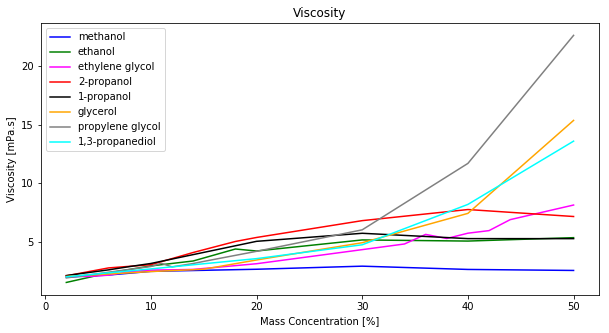
\includegraphics[width=1\textwidth]{visc.png}
    \centering
    \captionsetup{justification=centering}
    \caption{Viscosity Values of 8 Sample Alcohol Types Across Mass Concentration}
\end{figure}

In the viscosity graph, while all values converged to the value of pure water, 
which is expected, the viscosity line of methanol also decreased as methanol 
is less viscous than water.
\section{Model Result Analysis}
As mentioned in the method section, the training data will be defined in 5 
different ways: randomly divided, excluding all propylene glycol data, 
excluding all glycerol data, excluding all methanol data and excluding all 
2-propanol data. The result for each data division approach is presented as 
follows:
\begin{table}[ht]
    \centering
    \caption{Performance Score on the Testing Data Set}
    \begin{tabular}{|c|c|c|}
        \hline
        \hline
        Training Data & TC $R^2$ Score & Visc $R^2$ Score\\
        \hline
        Randomly divided & 0.96  & 0.70\\
        Propylene Glycol data excluded & 0.86  & 0.74\\
        Glycerol data excluded & 0.36  & 0.76\\
        Methanol data excluded & 0.92 & Failed\\
        2-propanol data excluded & 0.90  & 0.72\\
        \hline
    \end{tabular}
    \label{table:1}
\end{table}

The results indicate that for any alcohol that has structural similarities 
with data in the training set, has a high performance score when used on 
the testing data set. However, the alcohols that are significantly different 
from the training sets have a quite low performance scores.

For thermal conductivity models, except for glycerol-excluded approach model, 
all the models possess a decent performance score. The explanation for this is 
that the testing sets in such cases are similar to the training sets. While 
propylene glycol - 1,3-propanediol and 1-propanol - 2-propanol are pairs of 
structural isomers, methanol is also quite close to ethanol. However, even 
though the molecular structure of glycerol is not so distinguished to the 
others, it is the only type of alcohol that had the gradient of the thermal 
conductivity that trends significantly different from the others; not to 
mention that glycerol is the only type of alcohol that possesses 3 hydroxyl 
groups within the molecule. This helps to explain why the glycerol-excluded 
model performance score is quite low.

A similar explanation can be applied to explain the phenomenon in the 
viscosity models. In methanol-excluded model, the model failed to predict 
the viscosity values of methanol. Recalling the simulation data in the 
previous sub-section, methanol was the only type of alcohol that had a 
non-increasing value trend. It came from the fact that within the sample, 
methanol is the only type of alcohol that is less viscous than water. In 
other words, methanol is very different from the other alcohols when looking 
from a viscosity point of view. Thus, the model could not predict the 
viscosity values of methanol since it did not learn any methanol similar 
relationship during the training process. The other models have moderate 
performance scores but are not satisfactory. Since these models included 
methanol in the training process, it is likely that the bizarre viscosity 
of methanol influenced the prediction ability and resulted in non-satisfactory 
performance scores.

For future improvement of this method, the sample alcohol types should be 
diversified to obtain more generalized prediction models. Since low viscosity 
of methanol is a good point, we should include more alcohol types that are 
less viscous than water. However, there might be a chance that the selected 
variables are not sufficient to cover abnormal cases. Thus, independent 
research on how molecular structures influence the thermophysical properties 
of unusual alcohol types like methanol should be conducted to improve the 
variable sets. At the same time, we also need to diversify the sample in terms 
of structural features. Obviously, the sample alcohol types only have single 
bonds and straight carbon chain. Thus, the addition of double bonds, triple 
bonds, circle structures and tree-like carbon chain could help generalize the 
solutions.

While including methanol in the construction of models can give us a better 
direction to prepare data and investigate on a certain direction, I will 
exclude methanol out of the construction of the model in order to investigate 
the capability of this methodology for prediction when performance scores are 
sufficiently high. The expected performance score should be significantly 
higher than the previous version. Thus, the finalized models performance 
scores become
\begin{table}[ht]
    \centering
    \caption{Finalized Models Performance Scores}
    \begin{tabular}{|c|c|}
        \hline
        \hline
        Thermal Conductivity $R^2$ Score & Viscosity $R^2$ Score\\
        \hline
        0.96  & 0.91\\
        \hline
    \end{tabular}
    \label{table:2}
\end{table}

The models also help us to investigate how variables influence the 
thermophysical properties using the F-score method \cite{sasaki_truth_2007}. 
For the final models, the variable influences (feature importance) 
are as follows:

\begin{figure}[ht]
    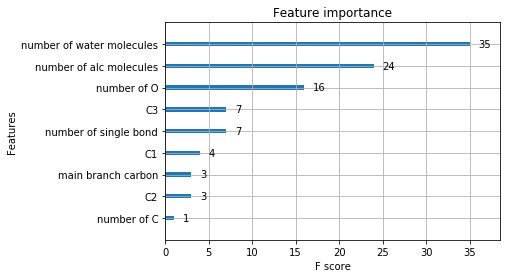
\includegraphics[width=1\textwidth]{fitc.png}
    \centering
    \captionsetup{justification=centering}
    \caption{Feature Importance of the Thermal Conductivity Model}
\end{figure}
\begin{figure}[ht]
    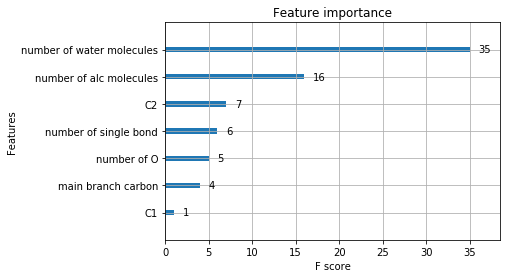
\includegraphics[width=1\textwidth]{fiv.png}
    \centering
    \captionsetup{justification=centering}
    \caption{Feature Importance of the Viscosity Model}
\end{figure}
\newpage

As expected, the mass concentration is one of the main factors that decides 
the thermal properties of the mixtures by having the number of water molecules 
and alcohol molecules as the highest influential variables. However, due to 
some noises and possibly the lack of better variables in the viscosity model, 
the score of the number of alcohol molecules is slightly underestimated or the 
score of the number of water molecules is slightly overestimated. Nonetheless 
the importance of these 2 variables are still clearly shown.\\
For thermal conductivity, another research \cite{manjunatha_investigation_2017} also showed that 
the number of hydroxyl groups affect the heat transfer ability of the alcohol. 
Interestingly, by using machine learning approach, we can also know that the 
hydroxyl group at the 3rd carbon position in the main carbon chain and the 
number of single bonds also have a significant influence on the thermal 
conductivity.\\
For viscosity, it is the hydroxyl group at the 2nd carbon position in the 
main carbon chain that significantly affect the viscosity values.

\section{Optimization Results}
Using the formulation \ref{eq:obj} and the related constraints, the results for 
optimization showed that the alcohol types with the following estimated 
structural features will have the optimal performance on both thermal 
conductivity and viscosity:
\begin{table}[ht]
    \centering
    \caption{Predicted Structural Features From Optimization}
    \begin{tabular}{|c|c|c|c|c|c|c|c|}
        \hline
        \hline
        \thead{Ratio of Molecules \\ (alcohol/water)} & \thead{Number of \\carbon} & \thead{Number of \\oxygen}
        & \thead{Number of \\single bond} & \thead{Length of \\(main) \\ (carbon chain)} & \thead{Position of \\hydroxyl \\groups}\\
        \hline
        0.0005-0.0148  & 3-4 & 3 & 13,17 & 3 & 1, 2, 3\\
        \hline
    \end{tabular}
    \label{table:opt}
\end{table}
\begin{table}[ht]
    \centering
    \caption{Predicted Thermophysical Properties From Optimization}
    \begin{tabular}{|c|c|}
        \hline
        \hline
        \thead{Predicted Thermal Conductivity\\ (W/m.K)}& \thead{Predicted Viscosity \\(mPa.s)}\\
        \hline
         0.81219405 & 2.0989997\\
        \hline
    \end{tabular}
    \label{table:prop}
\end{table}

As we can see, the best mixture is almost water, as water so far has the best 
thermal conductivity and viscosity. Furthermore, one of the molecular 
structures that can be constructed from these predicted features is glycerol, 
which is the type of alcohol that has the highest thermal conductivity and 
quite good viscosity across mass concentrations of alcohol-water mixtures 
according to the simulated data. This is showing that the methodology is 
approaching on the right direction. In the future work, with the additional 
constraint of freezing point, the method will be able to produce the desired 
outcome. Even though we obtained the features, the lack of diversity in terms 
of molecular structure from the sample data prevents us from constructing a 
complete structure. Thus, in the future where this method is applied, the 
sample data need to be sufficiently diverse enough as discussed in the 
previous sub-section. At the same time, an interpreting method should also be 
developed to translate from the broken down molecular structural features to 
a complete structure.